\chapter{Verification of Two Tension Cases from Allen and Wells (2014)} \label{chap:verification-allen-wells}

\begin{frame}
%\mode<article>{Content that only goes in the dissertation}
\mode<presentation>{Content that only goes in the slides.}
\end{frame}
\note{A set of notes.

\vfill

Split the notes by sentence.

\vfill

Leaves plenty of room between them for referring to while presenting.

\vfill
}

This chapter will show the development of a set of modeling tools to study surface cracks in flat plates, using FEACrack, Python, and WARP3D.
These tools were first used to verify two tension models from \citeauthor{allenwells2014} (\citeyear{allenwells2014}), and then to solve an intermediate case, demonstrating the limits of the interpolation methodology.
Details of the algorithms used in the Python programs are given in \Cref{chap:development-bending-models}.

\section{Identified Gaps in Interpolation Data}

\citeauthor{allenwells2014} built a set of 600 finite element models of surface cracks in tension, covering all combinations of
\begin{align*}
\frac{a}{t} &= 0.2, 0.4, 0.6, 0.8 & \frac{E}{\Sys} &= 100, 200, 300, 500, 700, 1000 \\
\frac{a}{c} &= 0.2, 0.4, 0.6, 0.8, 1.0 & n &= 3, 4, 6, 10, 20.
\end{align*}
Results for a set of models with \(\frac{a}{t}=0.6\) and \(n=6\) are shown in \Cref{fig:aspect-ratio-gap,fig:modulus-gap}.
The first figure shows a large gap between the results for cases \(\frac{a}{c}=0.2\) and \(\frac{a}{c}=0.4\), and the second figure shows a similar gap between the results for cases \(\frac{E}{\Sys}=100\) and \(\frac{E}{\Sys}=200\).
In each figure, normalized CMOD values for the more extreme case nearly double at comparable normalized stress levels, and the normalized \J values for the more extreme case are reduced by almost half at identical normalized CMOD levels.
As the authors use the solved models in a linear interpolation method, they identified a potential need for additional models with \(\frac{a}{c}=0.3\) and \(\frac{E}{\Sys}=150\), since there is no guarantee that the cracked plates exhibit linear behavior over such a wide range of results.
\begin{frame}
\begin{figure}[tbp]
%\forceversofloat
\centering
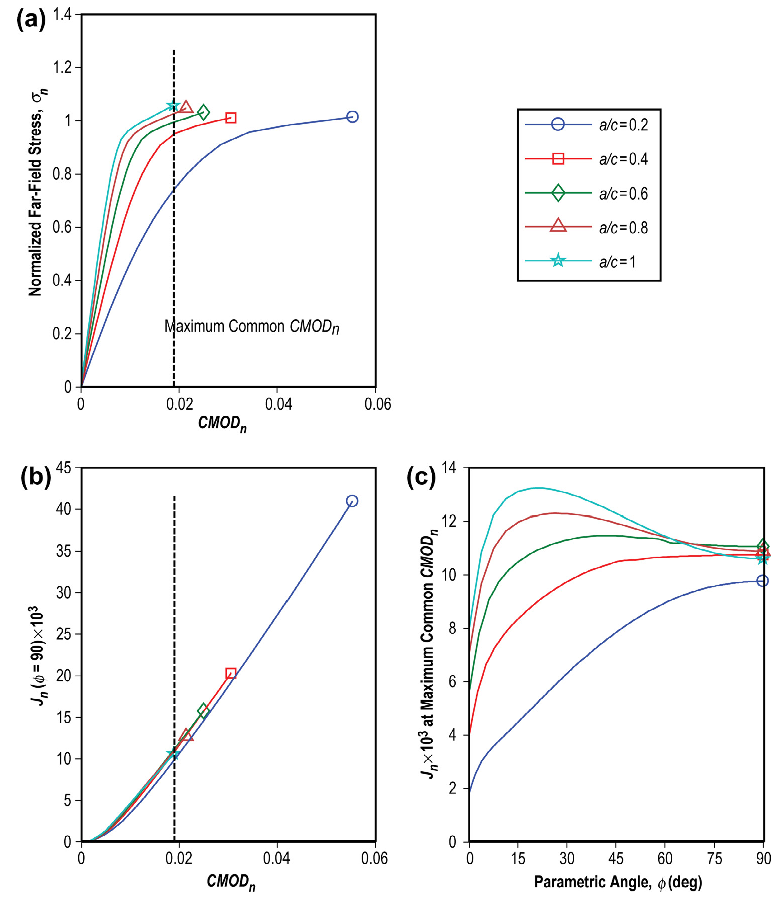
\includegraphics[width=0.7\columnwidth]{aspect-ratio-gap}
\caption{\label{fig:aspect-ratio-gap} Gap in results for very wide aspect ratios \citep{allenwells2014}}
\end{figure}
\begin{figure}[tbp]
\centering
%\forcerectofloat
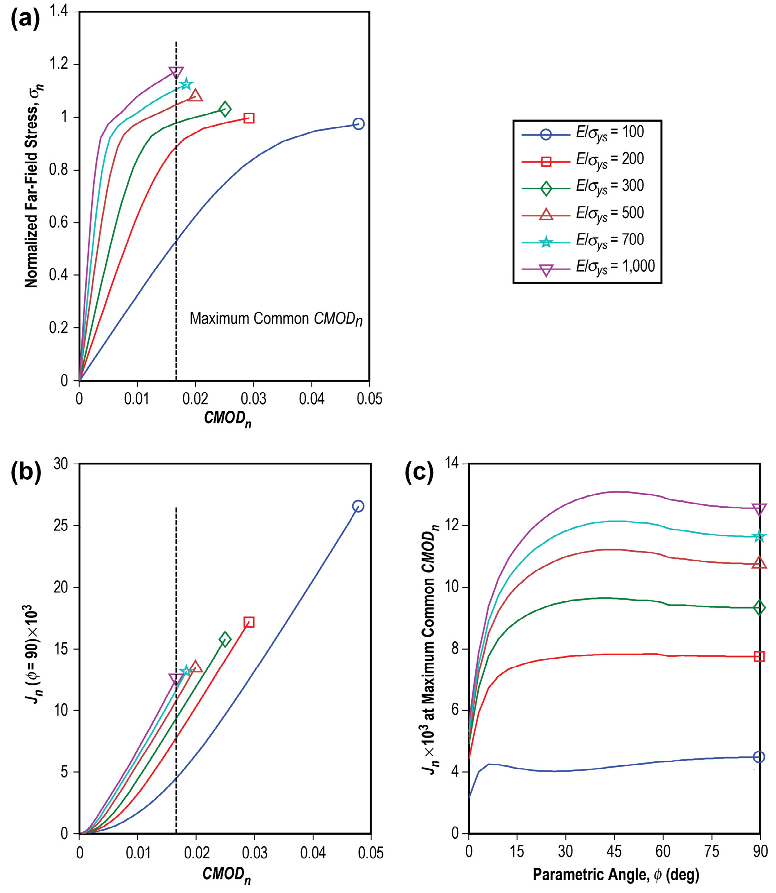
\includegraphics[width=0.7\columnwidth]{modulus-gap}
\caption{\label{fig:modulus-gap} Gap in results for very low elastic modulus values \citep{allenwells2014}}
\end{figure}
\end{frame}

\Cref{chap:app-verification-allen-wells} details the use of FEACrack \citep{feacrack} and WARP3D \citep{warp3d} to replicate the published results for the cases
\begin{align*}
\frac{a}{t} &= 0.6 & \frac{E}{\Sys} &= 100 \text{ and } 200\\
\frac{a}{c} &= 0.6 & n &= 6
\end{align*}
and the remainder of this chapter will show the results of a purpose-built model for \(\frac{E}{\Sys} = 150\) compared to an interpolated model using results from \(\frac{E}{\Sys}=100\) and \(\frac{E}{\Sys}=200\).

\section{Applying Procedure to New Material Model (\(\frac{E}{\Sys} = 150\))}

After modifying the \(\frac{E}{\Sys} = 200\) model from \Cref{chap:app-verification-allen-wells} to use \(E = 150\) and leaving the remote displacement at 0.0550, the new material model was solved.
As seen in \Cref{fig:e150_1}, the remote displacement was not high enough to place the model into the plastic regime, so the remote displacement was increased to 0.080.
The result of the new displacement is shown in \Cref{fig:e150_2}, and has clearly reached the plastic regime.
Later models used the secant method, and reached a CMOD of roughly 0.03.
\begin{frame}
\begin{figure}[tbp]
\centering
%\forcerectofloat
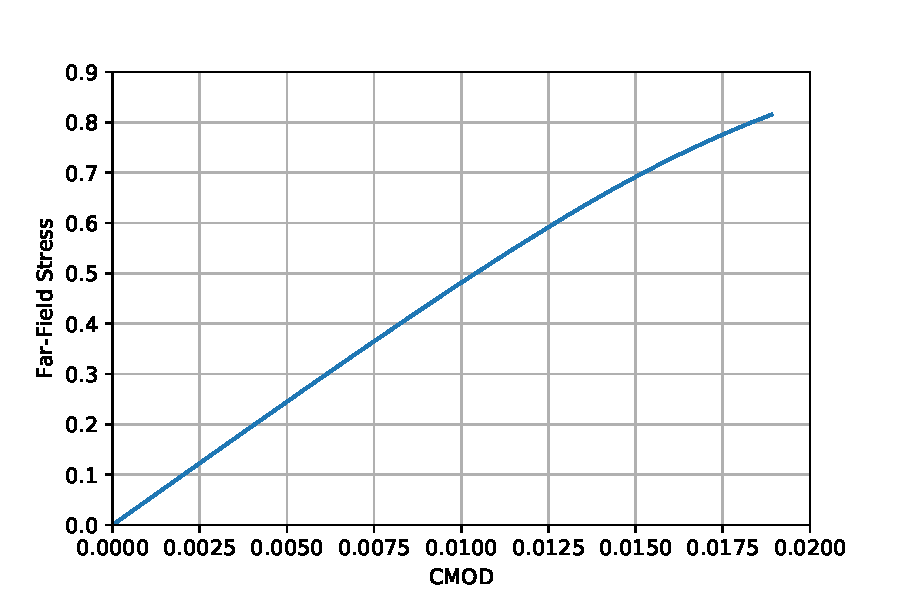
\includegraphics[width=0.8\columnwidth]{e150_1}
\caption{\label{fig:e150_1} First attempt at new material model}
\end{figure}
\end{frame}
\begin{frame}
\begin{figure}[tbp]
\centering
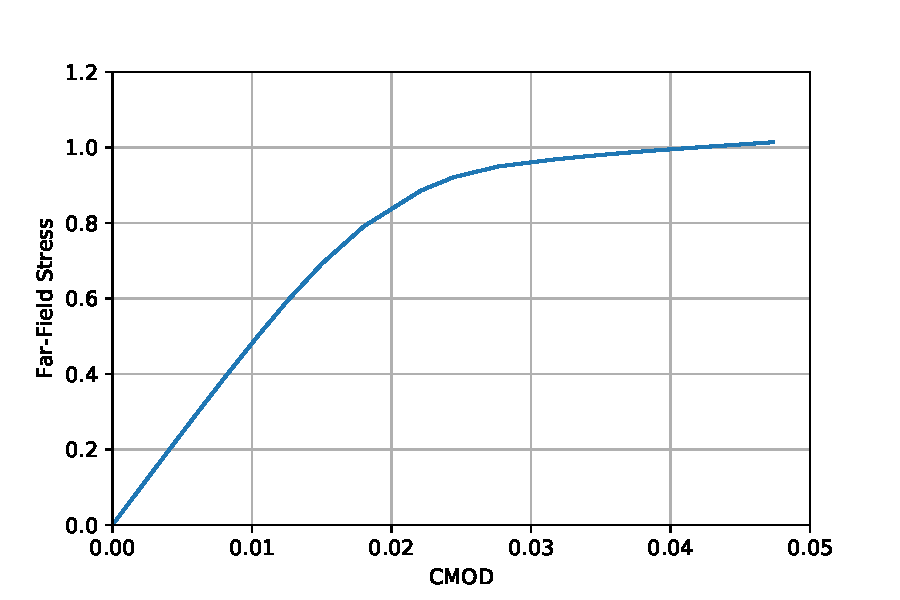
\includegraphics[width=0.8\columnwidth]{e150_2}
\caption{\label{fig:e150_2} Second attempt at new material model}
\end{figure}
\end{frame}

Finally, by comparing the \(\frac{E}{\Sys} = 150\) FEA results to the interpolated TASC result from \Cref{fig:tasc_interp_outputs}, we see that the FEA results are slightly more compliant in the elastic regime, and a sharper transition to the plastic regime at higher stress levels.
The two results differ by 5\% or less, as shown in \Cref{fig:e100_150_200_verification}.
\begin{frame}
\begin{figure}[tbp]
\centering
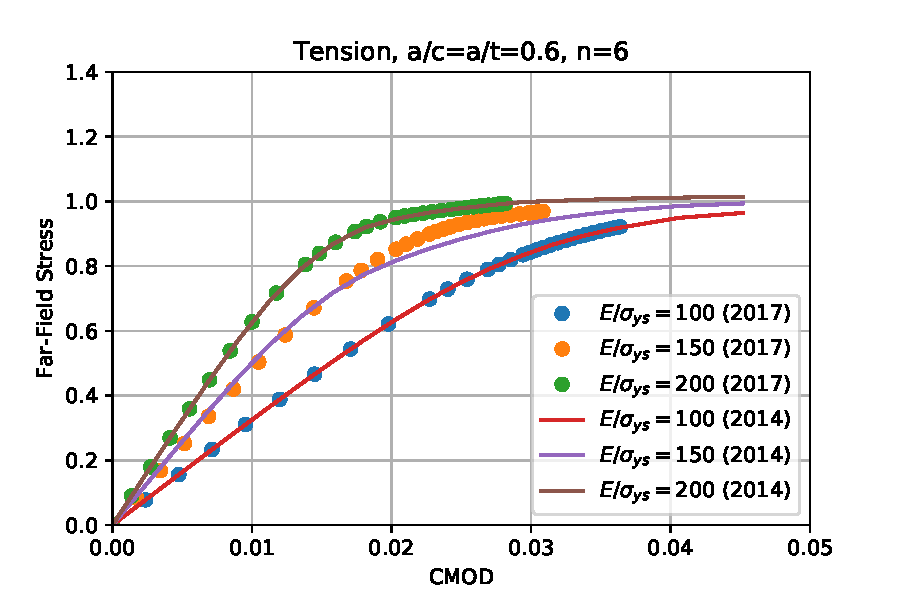
\includegraphics[width=0.8\columnwidth]{e100_150_200_verification}
\caption{\label{fig:e100_150_200_verification} Comparison of FEA result, interpolated result, and TASC raw data}
\end{figure}
\end{frame}

\section{Plotting CMOD, \J and \(\phi\)}

The final data to extract from the FEA results are values for the \J integral at each load increment. \J is a function of both load and position along the crack front, measured by the angle \(\phi\) from the free surface of the plate. \Cref{fig:j-phi-cmod-paa} shows an example of that function from \cite{allenwells2014}, and \Cref{fig:j-phi-cmod-mwr} shows a comparable function from the current models.

\begin{frame}
\begin{figure}[tbp]
\centering
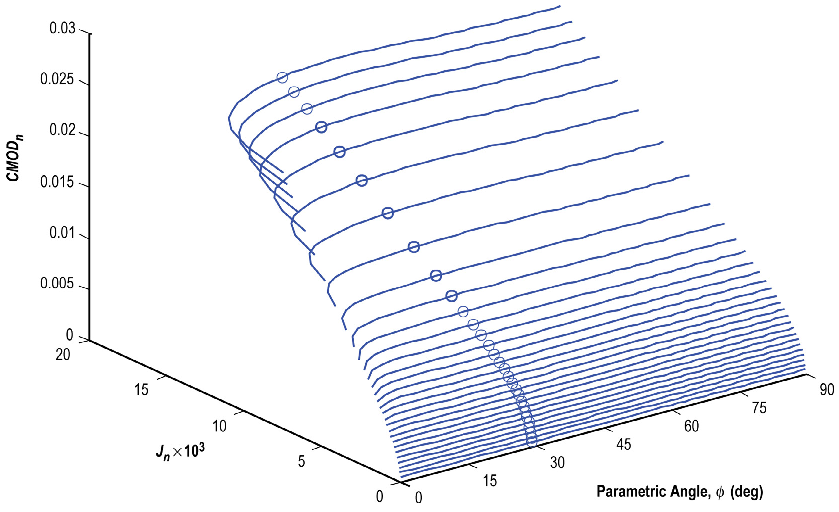
\includegraphics[width=0.8\columnwidth]{j-phi-cmod-paa}
\caption{\label{fig:j-phi-cmod-paa} Example relationship between \(\J(\phi)\) and CMOD \citep{allenwells2014}}
\end{figure}
\end{frame}

\begin{frame}
\begin{figure}[tbp]
\centering
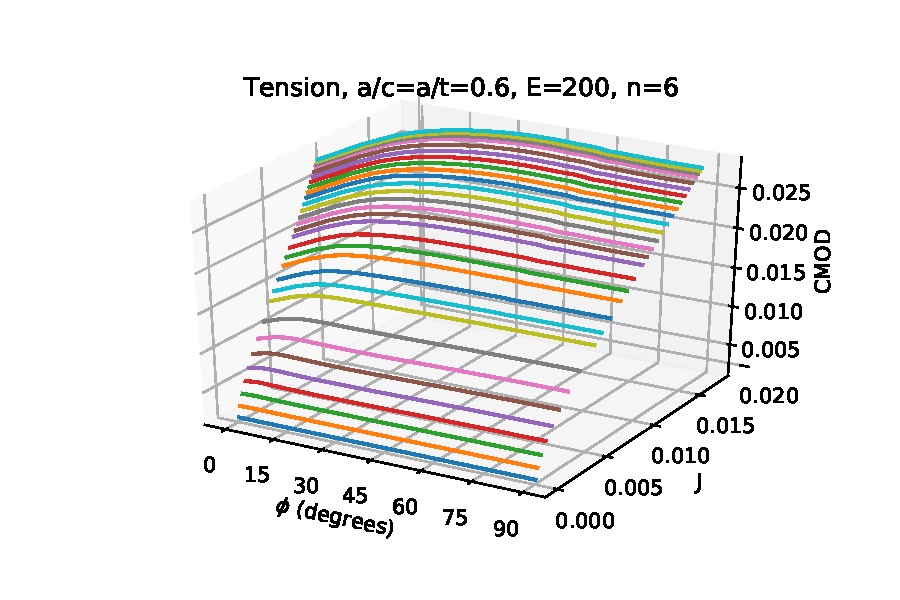
\includegraphics[width=0.8\columnwidth]{j-phi-cmod-mwr}
\caption{\label{fig:j-phi-cmod-mwr} Example relationship between \(\J(\phi)\) and CMOD}
\end{figure}
\end{frame}

%\begin{frame}[allowframebreaks]\mode<presentation>{\tiny}
%  \bibliography{cse_bibliography,v2}
%  \bibliographystyle{proposal}
%\end{frame}
